\documentclass[12pt]{report}
\usepackage[utf8]{inputenc}
\usepackage[english]{babel}
\usepackage{graphicx}
\usepackage{amssymb}
\usepackage{amsmath}
\usepackage{listings}
\usepackage{tikz}
\usepackage{float}
\PassOptionsToPackage{hyphens}{url}\usepackage{hyperref}
\usepackage[usestackEOL]{stackengine}
\usepackage{minted}

\usetikzlibrary{
    calc,trees,positioning,arrows,chains,shapes.geometric,%
    decorations.pathreplacing,decorations.pathmorphing,shapes,%
    matrix,shapes.symbols
}
\tikzset{
    block/.style={rectangle, rounded corners, minimum height=3em, draw=black, very thick,, text centered ,text width=7.5em},
    big_block/.style={rectangle, rounded corners, minimum height=3em, draw=black, very thick,, text centered ,text width=10em},
    line/.style={->, thick,shorten >=1.5pt},
    decoration={brace},
    tuborg/.style={decorate},
    tubnode/.style={midway, right=2pt},
}

\graphicspath{{images/}}

\title{Engineering a Programming Language}
\author{Èrik Campobadal Forés}

\begin{document}

\begin{titlepage}
    \begin{center}
        \vspace*{1cm}

        \huge
        \textbf{\thetitle}

        \vspace{0.5cm}

        \Large
        \thesubtitle

        \vspace{1.5cm}

        \textbf{\theauthor}

        \vfill

        \theintro

        \vspace{1cm}

        
\includegraphics[height=3.5cm]{upc}

        \vspace{1cm}

        \large

        \themeta

    \end{center}
\end{titlepage}


\tableofcontents
\listoffigures

\chapter{Introduction}
Programming languages are used every day by millions of engineers as part of their daily routine.
A programming language is used to tell a computer what to do. When
somebody wants a computer to do something, it needs to write a program using a programming language. Then,
a compiler needs to translate it into machine code to be executed.

To design a programming language it's important to understand the theory behind a compiler and to learn about all the
steps involved to make a computer understand and execute a program.

\section{Objectives}

The main objective of this thesis is to design an experimental programming language and implement an interpreter to execute
any program written with it. The different challenges that are faced during the design and implementation process are also explained and
solved in their respective chapters. The experimental language built in this thesis is called \emph{Nuua}.

The objective can be partitioned into the following points.

\begin{itemize}
    \item Learn all the steps involved in a common compiler implementation and reproduce them according to the project needs.
    \item Design the Nuua Programming Language. The grammar must be simple, elegant and yet it needs to follow the most
        common programming language's specifications to have a low learning curvature.
    \item Choose an efficient programming language to build the compiler and the interpreter with. Among other options, the languages that
    satisfy the previous statement are low-level programming languages like C \autocite{c_programming_language}, C++ \autocite{cpp_programming_language},
    D \autocite{d_programming_language}, Rust \autocite{rust_programming_language} or Go \autocite{go_programming_language} among others.
    \item Define a robust system architecture to design the compiler and the interpreter. The system architecture needs to be scalable.
    \item Build a compiler and an interpreter for the Nuua programming language and a very simple standard library.
\end{itemize}

\section{Preliminary overview}

This section briefly introduces some of the concepts found in this thesis, introducing preliminary concepts of language grammar, compilers and interpreters.
This preliminary overview won't deal with details and only explains the basics to understand the whole system without deep knowledge.
Further chapters contain expanded information respective to some of the details mentioned here.

\subsection{Language grammar}

Context-free grammar is a notation used to specify the syntax of a programming language. Following the syntax definition explained
in \autocite[Section~2.2]{compilers} a context-free grammar consists of four components:

\begin{enumerate}
    \item A group of terminal symbols also known as tokens. In a programming language tokens may be literal symbols like '+', '*' or numbers and identifiers.
    \item A group of non-terminals that can be reduced to terminals based on the production rules.
    \item A group of production rules that consists of a non-terminal on the left side and a sequence of terminals and/or non-terminals on the right side.
    \item A non-terminal start symbol.
\end{enumerate}

This thesis will use the \emph{extended Backus-Naur form} also known as \emph{EBNF} to express the context-free grammar representation of Nuua.
EBNF is often used in different ways due to the big amount of variants that exist. To EBNF syntax that this thesis is uses is shown in the
\autoref{fig:ebnf_syntax}. More information may be found in the EBNF grammar article \autocite{EBNF_grammar}.

\begin{table}[H]
    \centering
    \begin{tabular}{ l p{10cm} }
        \textbf{Symbol} & \textbf{Definition} \\
        \texttt{:} & Used to define a production rule. \\
        \texttt{\textit{space}} & Used to concatenate patterns (space separated). \\
        \texttt{A|B} & Used to define a union of A and B. \\
        \texttt{A+} & Used to define a one or more pattern of A. \\
        \texttt{A*} & Used to define a zero or more pattern. \\
        \texttt{A?} & Used to define an optional pattern. \\
        \texttt{(A)} & Used to group a pattern. \\
        \texttt{"T"} or \texttt{'T'} & Used to define a terminal symbol. \\
        \texttt{@A} & Used to indicate anything except A. \\
        \texttt{;} & Used to terminate a given production rule. \\
    \end{tabular}
    \caption{Variation of EBNF syntax used by this thesis}
    \label{fig:ebnf_syntax}
\end{table}

As a simple example, to define a language that consists of a single integer, the following EBNF grammar could be used:\\

\texttt{integer\\\tab: ("-" | "+")? digit+\\\tab;}\\
\texttt{digit\\\tab: "0"|"1"|"2"|"3"|"4"|"5"|"6"|"7"|"8"|"9"\\\tab;}\\

This variation is often used by many parser generators since it introduces a more visible and versatile approach to
write the language grammar.

\subsection{Compilers}

The job of a compiler is to take an input program written in a programming language and translate it into another as shown in \autoref{fig:compiler_overview}.
The compiler term is often used to express a translation to a much different level of abstraction, that usually means
that the input is written in a high-level language and further translated into another low-level language.

\begin{figure}[H]
    \centering
    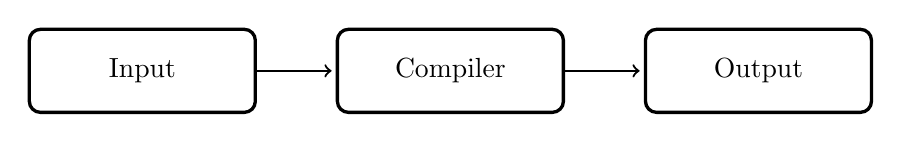
\begin{tikzpicture}
        [node distance=1cm]

        % Nodes of the layered system
        \node[block] (input) {Input};
        \node[block,right=of input] (compiler) {Compiler};
        \node[block,right=of compiler] (output) {Output};

        % Lines
        \draw[line] (input) -- (compiler);
        \draw[line] (compiler) -- (output);

    \end{tikzpicture}

    % Caption and Label
    \caption{Compiler overview}
    \label{fig:compiler_overview}
\end{figure}

\subsubsection{Phases of a compiler}

A compiler can also be decoupled into different parts. Each part does a very different job but they are all connected to each other.
In a typical compiler architecture, we may find all the different phases described in \autoref{fig:compiler_phases}.

Those phases are often found to be different depending on the implementation of the language. However, it's important to note what they do,
since they are often implemented in one way or another. More implementation details are explained in their respective chapters but in this
section, a small introduction to each phase is needed to understand the Nuua's system.

\begin{figure}[p]
    \centering
    \begin{tikzpicture}
        [node distance=1cm]

        \node (input) {Input};
        \node[bigger_block,below=of input] (lexical) {Lexical analysis (Lexer or scanner)};
        \node[bigger_block,below=of lexical] (syntax) {Syntax analysis (Parser)};
        \node[bigger_block,below=of syntax] (semantic) {Semantic analysis};
        \node[bigger_block,below=of semantic] (inter) {Intermediate code generator};
        \node[bigger_block,below=of inter] (opt) {Optimization};
        \node[bigger_block,below=of opt] (codegen) {Code generation};
        \node[below=of codegen] (output) {Output};

        \draw[line] (input) -- (lexical);
        \draw[line] (lexical) -- (syntax);
        \draw[line] (syntax) -- (semantic);
        \draw[line] (semantic) -- (inter);
        \draw[line] (inter) -- (opt);
        \draw[line] (opt) -- (codegen);
        \draw[line] (codegen) -- (output);

        % The right specifiers
        \draw[tuborg, decoration={brace}] let \p1=(lexical.north), \p2=(semantic.south) in
            ($(3.5, \y1)$) -- ($(3.5, \y2)$) node[tubnode] {Front end};
        \draw[tuborg, decoration={brace}] let \p1=(inter.north), \p2=(opt.south) in
            ($(3.5, \y1)$) -- ($(3.5, \y2)$) node[tubnode] {Middle end};
        \draw[tuborg, decoration={brace}] let \p1=(codegen.north), \p2=(codegen.south) in
            ($(3.5, \y1)$) -- ($(3.5, \y2)$) node[tubnode] {Back end};
    \end{tikzpicture}

    % Caption and Label
    \caption{Common compiler phases}
    \label{fig:compiler_phases}
\end{figure}

\begin{itemize}
    \item \emph{Lexical analysis}: In this phase, the input source is transformed from a character string into a token list, this is also called
        tokenization. Lexemes found in the source program are translated into individual tokens using different patterns. For example, some tokens
        might include integers, symbols (+, -, *, etc.), identifiers or keywords ('if', 'while', etc.).
    \item \emph{Syntax analysis}: In this phase, the implementation may vary among compilers, some of them work close to the lexical analysis since they
        can work together. However, its purpose is to perform operations given the token list to parse the input and create an Abstract Syntax Tree
        (AST). As seen in \autocite[Section~5.2.1]{engineering_a_compiler}, an AST is a data structure that represents the input program.
        (AST). As seen in \autocite[Section~5.2.1]{engineering_a_compiler}, an AST is a data structure that represents the input program.
        This stage determines if it's a valid program based on the language grammar and the specified rules.
        There are also scanner-less parsers that take the lexical analysis and the syntax analysis into a single step. It is harder to understand and
        debug compared to the modularity of splitting these two phases but it has some advantages like removing the token classification as mentioned
        in \autocite{scannerless_parsing}.
    \item \emph{Semantic analysis}: This phase analyzes the AST and creates a symbol table while analyzes the input source with things like type checking or
        variable declarations, if some operations can be performed (for example adding a number with a string). A symbol table is a structure used
        by further phases to see information attached to specific source code parts. For example, it can store information about a variable
        (if it's global, exported, etc.).
    \item \emph{Intermediate code generator}: An Intermediate representation (IR) can be avoided but it's often used to have a platform independent
        optimizer. Usually the code generation targets a specific architecture and would require different optimizers depending on each architecture.
        However, by having an IR it's possible to have a single optimizer. A much used IR is Three Address Code
        (TAC) that can be organized in quadruples or triples as seen by some examples in \autocite{three_address_code_examples}.
    \item \emph{Optimization}: This optimization is often performed on the IR and performs different tasks to allow a faster and smaller output. For example, it may
        remove dead code, perform loop optimizations, etc.
    \item \emph{Code generation}: This is where the real translation takes place, it translates the IR into a different language output. For example machine code.
        This phase often has to deal with instruction scheduling or register allocation while they have to output a fully working program.
\end{itemize}

\subsection{Interpreters}

There are different ways to interpret a program. Among the most popular options we can find a bytecode interpreter and an AST interpreter.

\begin{itemize}
    \item \emph{Bytecode interpreter}: The program is first compiled to bytecode instructions and further interpreted. Bytecode interpreters are often
        implemented as virtual machines since most of the times bytecode instructions are very similar to real hardware instructions.
        The usual choices are stack or register machines. There have been many discussions on the advantages and the inconveniences of both of them, more information may be seen at \autocite{stack_vs_register}. An example of a virtual machine is the Lua virtual machine \autocite{the_implementation_of_lua}.
    \item \emph{Abstract syntax tree interpreter}: This kind of interpreters just need the AST to work with, so no extra compilation to bytecode
        is needed and therefore, they are easier to implement. However, due it's nature, they are much slower to execute and debug due to the recursiveness of working with tree data structures.
\end{itemize}

\subsection{Just-in-time compilers}

Just-in-time compilers (often called JIT compilers) are an intermediate approach between a compiler that generates machine code and an interpreter.
JIT compilers compile chunks of code at specific moments while the program run to speed up portions of the code that is being interpreted
(for example functions that are called frequently). Essentially, the JIT compiler needs to decide when to compile a specific part of the code at
runtime and adds a small overhead in exchange for a machine-language performance on specific parts of the program.

More information about JIT compilers and the tools that can be used can be found at \autocite{jit_compilation}.

\section{System architecture}
\label{sec:sys_arch}

To design the system architecture of Nuua, consideration of existing system architectures needs to be taken since existing architectures
often work better than the custom-made ones and they often lead to greater project scalability. It's trivial
to make this choice before starting the project since changing a system architecture after it's initial
development phases becomes a very bad choice and may lead to a big ball of mud. Two choices in software development might be hierarchical
or layered systems. Nuua's architecture is based on a \emph{layered system} \autocite{software_architecture}.

A layered system has specific requirements regarding code communication. Specifically, a layered system consists
of different layers arranged vertically. Those layers have a specific criterion that needs to be met. As a matter of fact,
each layer can only use the layer below and gives an API for the layer above (if any) to use its functions. For example,
the \autoref{fig:layered_system} shows a simple 3-tier layered system. Layer 3 can only use Layer 2, and the output comes
from Layer 2. Layer 3 cannot use Layer 1 nor expect any outputs from it. It's the Layer 2 responsibility to use the Layer 1
and process its output before it can give its own output.

\begin{figure}[H]
    \centering
    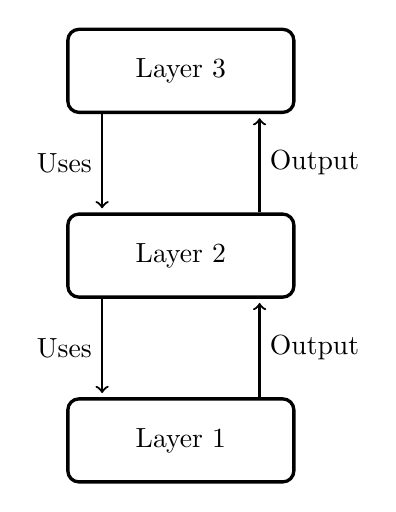
\begin{tikzpicture}
        [node distance=1.25cm]

        % Nodes of the layered system
        \node[block] (layerc) {Layer 3};
        \node[block,below=of layerc] (layerb) {Layer 2};
        \node[block,below=of layerb] (layera) {Layer 1};

        % Arrows going down
        \draw[line] ($(layerc.south) + (-1, 0)$) -- node[midway, left] {Uses} ($(layerb.north) + (-1, 0)$);
        \draw[line] ($(layerb.south) + (-1, 0)$) -- node[midway, left] {Uses} ($(layera.north) + (-1, 0)$);

        % Arrows going up
        \draw[line] ($(layerb.north) + (1, 0)$) -- node[midway, right] {Output} ($(layerc.south) + (1, 0)$);
        \draw[line] ($(layera.north) + (1, 0)$) -- node[midway, right] {Output} ($(layerb.south) + (1, 0)$);

    \end{tikzpicture}

    % Caption and Label
    \caption{Layered system}
    \label{fig:layered_system}
\end{figure}

This system is known to be robust, easy to test and with a high ease of development as mentioned in \autocite{software_architecture_patterns}.
It's very easy to understand and a widely used system. This system is also used for other complex software systems,
such as operating systems or complex protocols like TCP/IP.

By using a layered system each layer gets completely isolated and works independently by just using the layer below,
creating a way to scale-up or upgrade existing parts of the system without damaging the others. This introduces a
very powerful \emph{separation of concerns} among all the system layers since each layer has a specific role and only deals
with the logic that pertains to it.
However, a consistent API should, in fact, be established from the ground up to avoid backward incompatible changes.
If the API is maintained, the individual layers may be upgraded independently without the need for extra work.

\autoref{fig:nuua_system} shows the Nuua architecture. An independent module called Logger is found
on the left side of the figure. This module is a logger used by all layers to output messages if needed (for example error reporting).

\begin{figure}[p]
    \centering
    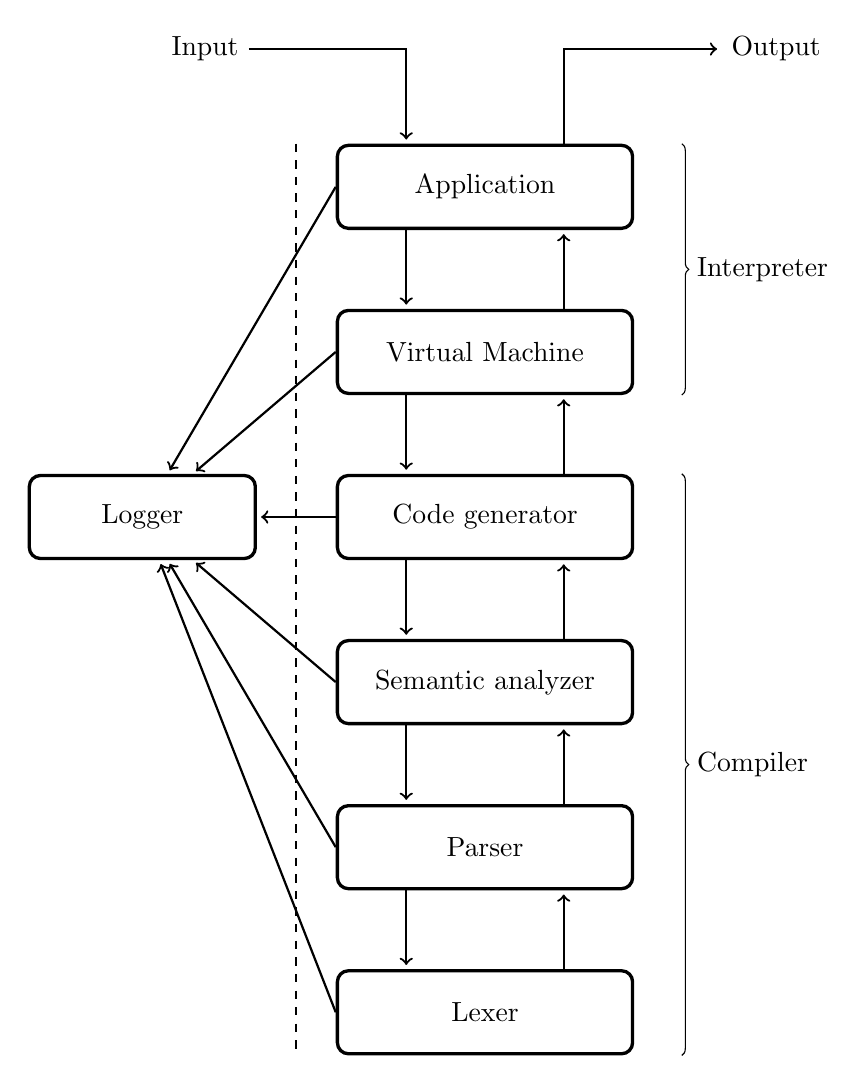
\begin{tikzpicture}
        [node distance=1cm]

        % Nodes of the layered system
        \node[big_block] (app) {Application};
        \node[big_block,below=of app] (vm) {Virtual Machine};
        \node[big_block,below=of vm] (compiler) {Code generator};
        \node[big_block,below=of compiler] (analyzer) {Semantic analyzer};
        \node[big_block,below=of analyzer] (parser) {Parser};
        \node[big_block,below=of parser] (lexer) {Lexer};

        % Independent module
        \node[block, left=of compiler] (logger) {Logger};

        % Separator
        \draw[thick,dashed] ($(app.north west) + (-0.5, 0)$) -- ($(lexer.south west) + (-0.5, 0)$);

        % Top arrows
        \draw[line] (-3, 1.75) node[anchor=east] {Input} -| ($(app.north) + (-1, 0)$);
        \draw[line] ($(app.north) + (1, 0)$) |- (3, 1.75) node[anchor=west] {Output};

        % Arrows going down
        \draw[line] ($(app.south) + (-1, 0)$) -- ($(vm.north) + (-1, 0)$);
        \draw[line] ($(vm.south) + (-1, 0)$) -- ($(compiler.north) + (-1, 0)$);
        \draw[line] ($(compiler.south) + (-1, 0)$) -- ($(analyzer.north) + (-1, 0)$);
        \draw[line] ($(analyzer.south) + (-1, 0)$) -- ($(parser.north) + (-1, 0)$);
        \draw[line] ($(parser.south) + (-1, 0)$) -- ($(lexer.north) + (-1, 0)$);

        % Arrows going up
        \draw[line] ($(vm.north) + (1, 0)$) -- ($(app.south) + (1, 0)$);
        \draw[line] ($(compiler.north) + (1, 0)$) -- ($(vm.south) + (1, 0)$);
        \draw[line] ($(analyzer.north) + (1, 0)$) -- ($(compiler.south) + (1, 0)$);
        \draw[line] ($(parser.north) + (1, 0)$) -- ($(analyzer.south) + (1, 0)$);
        \draw[line] ($(lexer.north) + (1, 0)$) -- ($(parser.south) + (1, 0)$);

        % Logger arrows
        \draw[line] (app.west) -- (logger);
        \draw[line] (vm.west) -- (logger);
        \draw[line] (compiler.west) -- (logger);
        \draw[line] (analyzer.west) -- (logger);
        \draw[line] (parser.west) -- (logger);
        \draw[line] (lexer.west) -- (logger);

        % The right specifiers
        \draw[tuborg, decoration={brace}] let \p1=(app.north), \p2=(vm.south) in
            ($(2.5, \y1)$) -- ($(2.5, \y2)$) node[tubnode] {Interpreter};
        \draw[tuborg, decoration={brace}] let \p1=(compiler.north), \p2=(lexer.south) in
            ($(2.5, \y1)$) -- ($(2.5, \y2)$) node[tubnode] {Compiler};
    \end{tikzpicture}

    % Caption and Label
    \caption{Nuua's architecture diagram (Layered System)}
    \label{fig:nuua_system}
\end{figure}

\begin{itemize}
    \item \emph{Logger}: Used by all layers to debug or log errors. In case of a fatal error, the logger outputs
        an error stack in a fancy way and terminates the application.
    \item \emph{Application}: This layer is used to decode the command line arguments and fire up the compiler toolchain. In short,
        the purpose is to analyze the command line arguments and fire the application accordingly.
    \item \emph{Virtual Machine}: The virtual machine is the interpreter that runs Nuua. It's a register-based virtual machine that
        acts as the Nuua runtime environment.
    \item \emph{Code generator}: Is responsible for the translation of the AST to the virtual machine bytecode. This acts as the code generation
        part of a compiler architecture.
    \item \emph{Semantic analyzer}: Does all the semantic analysis of the compiler and optimizes the AST for faster and smaller output.
    \item \emph{Parser}: Acts as the syntax analyzer, it uses a list of tokens and generates a fully valid AST.
    \item \emph{Lexer}: Scans the source code and translates the characters to tokens, creating a list of tokens representing
        the original source code.
\end{itemize}


\chapter{The Nuua Language}
This chapter defines the Nuua programming language. Nuua is a general purpose programming language with an imperative
paradigm and a statically typed system. The Nuua compiler and virtual machine explained in this thesis are written in C++
with a zero-dependency policy. The interpreter is a register-based bytecode virtual machine.

Nuua's system architecture built in this thesis, as described in \autoref{sec:sys_arch}, consists of a compiler that translates a program written
in Nuua into bytecode instructions and of a virtual machine interpreter that executes those bytecode instructions.

\section{Grammar}

Nuua's grammar is inspired by other existing programming languages by taking advantage of some of the best features some of them offer.
Inspiration comes especially from Python \autocite{python_programming_language}, Rust \autocite{rust_programming_language} and
Go \autocite{go_programming_language}.

The precedence relationship between expressions is heavily inspired by C \autocite{c_programming_language}, D \autocite{d_programming_language},
Rust \autocite{rust_programming_language}, and Dart \autocite{dart_programming_language}. The official documentation for those languages
exposes similar tables for operator precedences and Nuua has taken akin levels of precedence as those.

Nuua does not make use of the \texttt{";"} to separate statements, instead, it uses the same separator as Go. Statements can be separated by
a \texttt{"\textbackslash n"} but it does not make use of the \texttt{"\textbackslash t"} to indicate statements inside blocks, and uses the typical
block separator \texttt{"\{" ... "\}"}.

\subsection{Lexical Grammar}

Lexical grammar is used by the lowest layer of the Nuua system to scan the source language and identify different terminal symbols.
The main difference with the syntax grammar, as exposed in \autocite[Appendix~I]{crafting_interpreters}, is that the syntax grammar is a context-free grammar and lexical grammar is a regular grammar.

Nuua's lexical rules are as follows:

\begin{lstlisting}
DIGIT
    : "0" | ... | "9"
    ;
\end{lstlisting}

Digits are any character from '0' to '9'.

\begin{lstlisting}
ALPHA
    : "a" | ... | "z"
    | "A" | ... | "Z"
    | "_"
    ;
\end{lstlisting}

Alpha are characters that are part of the English alphabet in lower or upper case. It also includes '\_' as a special character.

\begin{lstlisting}
ALPHANUM
    : DIGIT
    | ALPHA
    ;
\end{lstlisting}

Alphanum are characters that are either part of the alphabet or are digits.

\begin{lstlisting}
INTEGER_EXPR
    : DIGIT+
    ;
\end{lstlisting}

Integers are a single digit or more found sequentially without spaces. The integer sign is not represented here.

\begin{lstlisting}
FLOAT_EXPR
    : DIGIT+ "." DIGIT+
    ;
\end{lstlisting}

Floats are like integers but require a dot followed by a digit or more, creating a decimal number.

\begin{lstlisting}
BOOL_EXPR
    : "true"
    | "false"
    ;
\end{lstlisting}

Bools are either 'true' or 'false', that are keywords.

\begin{lstlisting}
STRING_EXPR
    : '"' @'"' '"'
    ;
\end{lstlisting}

Strings represent a character string with the possibility to escape '"' by using a '\textbackslash' as a prefix, more on that in the upcoming sections.

\begin{lstlisting}
IDENTIFIER
    : ALPHA ALPHANUM*
    ;
\end{lstlisting}

Identifiers are an alpha character followed by an optional one or more alphanumeric character.

\subsection{Syntax Grammar}

The syntax grammar is used by the parser to build the abstract syntax tree that determines the program's execution flow.
These rules include all top-level declarations, statements, and expressions.

\subsubsection{Program and Top Level Declarations}
\label{sec:program_tld}

\begin{lstlisting}
program
    : top_level_declaration*
    ;
\end{lstlisting}

A Nuua program is a list of top-level declarations.

\begin{lstlisting}
top_level_declaration
    : use_declaration "\n"
    | fun_declaration "\n"
    | class_declaration "\n"
    | export_declaration "\n"
    ;
\end{lstlisting}

A top-level declaration can only be one of the specified rules. Top-level declarations are
a special type of declaration that can only be declared on the module and not inside other blocks.

\begin{lstlisting}
use_declaration
    : "use" STRING_EXPR
    | "use" IDENTIFIER ("," IDENTIFIER)* "from" STRING_EXPR
    ;
\end{lstlisting}

A use declaration is used to import other top-level declarations from other modules. By using the first rule, Nuua imports all the
exported targets of the module pointed by STRING\_EXPR. Otherwise, Nuua imports the specified targets from the modules.

\begin{lstlisting}
fun_declaration
    : "fun" IDENTIFIER "(" parameters? ")" (":" type)? fun_body;
    ;
parameters
    : variable_declaration ("," variable_declaration)*
    ;
fun_body
    : "->" expression "\n"
    | "=>" statement
    | "{" "\n" statement* "}" "\n"
    ;
\end{lstlisting}

A function is defined using the keyword \texttt{fun} followed by the function name, and a list of optional parameters enclosed in parentheses.
The function type is specified after the parameter list by using \texttt{:}. The return type might not be present if the function has no return value.
The function body is specified in three different ways depending on the type of the function body that is expected.

\begin{lstlisting}
class_declaration
    : "class" "{" class_statement* "}"
    ;
class_statement
    : variable_declaration
    | fun_declaration
    ;
\end{lstlisting}

A class uses a keyword \texttt{class} and expects zero or more class statements.

\begin{lstlisting}
export_declaration
    : "export" top_level_declaration
    ;
\end{lstlisting}

An export declaration marks the following top-level declaration as exported, making it available for other modules to import it using the
use declaration.

\begin{lstlisting}
statement
    : variable_declaration "\n"
    | if_statement "\n"
    | while_statement "\n"
    | for_statement "\n"
    | return_statement "\n"
    | print_statement "\n"
    | expression_statement "\n"
    ;
\end{lstlisting}

Statements are used to change the program's flow or indicate simple actions like declaring a variable.

\begin{lstlisting}
variable_declaration
    : IDENTIFIER ":" type
    | IDENTIFIER ":" type "=" expression
    | IDENTIFIER ":" "=" expression
    ;
\end{lstlisting}

A variable declaration may have a type assigned with it, or the declaration type will be inferred from the initializer.

\begin{lstlisting}
if_statement
    : "if" expression if_body el_if* else?
    ;
if_body
    : "=>" statement "\n"
    | "{" "\n" statement* "}"
    ;
el_if
    : "elif" expression if_body
    ;
else
    : "else" expression if_body
    ;
\end{lstlisting}

An \texttt{if} statement is declared with the \texttt{if} keyword followed by the expression of its condition.
The \texttt{if} body may be declared in two different ways depending on the if body. The \texttt{elif} word may be used as a shorthand
to an \texttt{else} followed by an "if" inside. An optional \texttt{else} condition may be added at the end of the \texttt{if}.

\begin{lstlisting}
while_statement
    : "while" expression while_body
    ;
while_body
    : "=>" statement "\n"
    | "{" "\n" statement* "}"
    ;
\end{lstlisting}

A \texttt{while} statement uses the \texttt{while} keyword followed by the expression of the condition and the \texttt{while} body, that can be specified
in two different ways depending on the body contents.

\begin{lstlisting}
for_statement
    : "for" IDENTIFIER ("," IDENTIFIER)? "in" expression for_body
    ;
for_body
    : "=>" statement
    | "{" "\n" statement* "}"
    ;
\end{lstlisting}

A \texttt{for} statement acts is a way to interate a nuua iterator \autoref{fig:nuua_iterators}.
It gets declared by using the \texttt{for} keyword followed by an identifier that will be used to store the element
in the iterator. An optional second identifier may be given in case the loop index needs to be stored as well.
Those values change in every iteration. After the identifiers, the \texttt{in} keyword is expected, followed by the iterator expression and the
\texttt{for} body, that can be declared in two different ways depending on its content.

\begin{lstlisting}
return_statement
    : "return" expression?
    ;
\end{lstlisting}

A \texttt{return} statement uses the \texttt{return} keyword and an optional expression to return.

\begin{lstlisting}
print_statement
    : "print" expression?
    ;
\end{lstlisting}

The \texttt{print} expression is a statement that outputs an expression to the screen. This is a temporary statement used while
Nuua is not able to properly read and write to files (stdout / stdin) in this specific case.

\begin{lstlisting}
expression_statement
    : expression
    ;
\end{lstlisting}

An expression statement may be used as an expression whose value is not used or no value is returned from it.

\subsubsection{Expressions}
\label{sec:grammar_expressions}

Expressions are grouped in different production rules depending on their precedence, this is done due to the parsing strategy used and
helps to visualize the precedence by reading the grammar.

\begin{lstlisting}
expression
    : assignment
    ;
\end{lstlisting}

An expression is reduced to an assignment.

\begin{lstlisting}
assignment
    : range ("=" range)*
    ;
\end{lstlisting}

An assignment expression is written by an expression on the left-hand side and on the right-hand side with a \texttt{=} in the middle.

\begin{lstlisting}
range
    : logical_or ((".." | "...") logical_or)*
    ;
\end{lstlisting}

A range expression is written by an expression on the left-hand side and on the right-hand side with a \texttt{..} or \texttt{...} in the middle. Depending
if the range is exclusive or inclusive.

\begin{lstlisting}
logical_or
    : logical_and ("or" logical_and)*
    ;
\end{lstlisting}

A logical \texttt{or} is a binary operation with the keyword \texttt{or} in the middle.

\begin{lstlisting}
logical_and
    : equality ("and" equality)*
    ;
\end{lstlisting}

A logical \texttt{and} is a binary operation with the keyword \texttt{and} in the middle.

\begin{lstlisting}
equality
    : comparison (("!=" | "==") comparison)*
    ;
\end{lstlisting}

An equality comparison is a binary operation with a \texttt{!=} or \texttt{==} in the middle depending if the check needs to be negated or not.

\begin{lstlisting}
comparison
    : addition ((">" | ">=" | "<" | "<=") addition)*
    ;
\end{lstlisting}

A comparison is similar to equality but checks the values to determine if the left-hand side is greater, greater than, lower and lower than the
right-hand side.

\begin{lstlisting}
addition
    : multiplication (("-" | "+") multiplication)*
    ;
\end{lstlisting}

An addition is used to perform an addition or subtraction of two values.

\begin{lstlisting}
multiplication
    : cast (("/" | "*") cast)*
    ;
\end{lstlisting}

Multiplication is used to perform multiplication or division of two values.

\begin{lstlisting}
cast
    : unary_prefix ("as" type)*
    ;
\end{lstlisting}

A cast performs a type cast of the values on the left-hand side to the value of the right-hand side by using the \texttt{as} keyword.

\begin{lstlisting}
unary_prefix
    : ("!" | "+" | "-") unary_prefix
    | unary_postfix
    ;
\end{lstlisting}

The unary prefixes are used to change a value state by prefixing the operation.

\begin{lstlisting}
unary_postfix
    : primary unary_p*
    ;
unary_p
    : "[" expression "]"
    | slice
    | "(" arguments? ")"
    | "." IDENTIFIER;
    ;
slice
    : "[" expression? ":" expression? (":" expression?)? "]"
    ;
arguments
    : expression ("," expression)*
    ;
\end{lstlisting}

The unary postfixes are used to either access a value or mutate it's content, to slice it's contents, to call a value or to access a value property.

\begin{lstlisting}
primary
    : BOOL_EXPR
    | INTEGER_EXPR
    | FLOAT_EXPR
    | STRING_EXPR
    | IDENTIFIER
    | LIST_EXPR
    | DICTIONARY_EXPR
    | OBJECT_EXPR
    | "(" expression ")"
    ;
\end{lstlisting}

Primary expressions have the highest precedence and are mostly native types, with the exception of the expression group.

\begin{lstlisting}
OBJECT_EXPR
    : IDENTIFIER "{" object_args? "}"
    ;
object_args
    : IDENTIFIER ":" expression ("," IDENTIFIER ":" expression)*
    ;
\end{lstlisting}

An object is defined by an identifier containing the class name, followed by optional arguments surrounded by \texttt{\{} and \texttt{\}} to
initialize the class properties.

\begin{lstlisting}
LIST_EXPR
    : "[" expression ("," expression)* "]"
    ;
\end{lstlisting}

Lists can't be empty, so at least one expression must be provided.

\begin{lstlisting}
DICTIONARY_EXPR
    : "{" IDENTIFIER ":" expression ("," IDENTIFIER ":" expression)* "}"
    ;
\end{lstlisting}

Dictionaries, like lists, can't be empty, so at least one expression must be provided.

\subsection{Operator Precedence}

Given that expressions are grouped by their precedence, the operator precedence table of Nuua is as follows:

\begin{table}[H]
    \centering
    \begin{tabular}{ l l l }
        \textbf{Level} & \textbf{Operators} & \textbf{Associativity} \\
        \texttt{1} & \texttt{A[B], A[B:C:D], A(B, C, D, ...), A.B} & Left-to-right \\
        \texttt{2} & \texttt{!A, +A, -A} & Right-to-left \\
        \texttt{3} & \texttt{A as B} & Left-to-right \\
        \texttt{4} & \texttt{A/B, A*B} & Left-to-right \\
        \texttt{5} & \texttt{+A, -A} & Left-to-right \\
        \texttt{6} & \texttt{A\textgreater B, A\textgreater =B, A\textless B, A\textless =B} & Left-to-right \\
        \texttt{7} & \texttt{A!=B, A==B} & Left-to-right \\
        \texttt{8} & \texttt{A and B} & Left-to-right \\
        \texttt{9} & \texttt{A or B} & Left-to-right \\
        \texttt{10} & \texttt{A..B, A...B} & Left-to-right \\
        \texttt{11} & \texttt{A=B} & Right-to-left \\
    \end{tabular}
    \caption{Nuua operator precedence from highest to lowest with the associativity}
    \label{fig:nuua_operator_precedence}
\end{table}

\subsection{Keywords and Reserved Words}

Keywords are a special subset of identifiers that have a special meaning in a Nuua program.
A reserved word is an identifier that can't be used as such, and in Nuua, no keywords can be used as identifiers therefore
making all keywords reserved words at the same time.
All keywords can already be identified by looking at the grammar rules, the following list shows
all of the keywords in Nuua.\\

\begin{tasks}[counter-format = (tsk[r]), label-width = 2.5cm](4)
        \task \texttt{true}
        \task \texttt{false}
        \task \texttt{as}
        \task \texttt{or}
        \task \texttt{and}
        \task \texttt{if}
        \task \texttt{else}
        \task \texttt{for}
        \task \texttt{in}
        \task \texttt{while}
        \task \texttt{return}
        \task \texttt{print}
        \task \texttt{class}
        \task \texttt{fun}
        \task \texttt{use}
        \task \texttt{from}
        \task \texttt{elif}
        \task \texttt{export}\\
\end{tasks}

More information about the \texttt{print} keyword and why it does exist can be found in \autoref{sec:print_statement}.

\section{Scopes}
\label{sec:nuua_scopes}

Scopes refer to the visible area of the variables, in other words, it determines where the association between a variable name
and its value (known as name binding) is valid. This area is known as a scope block.

Nuua have two levels of scope blocks:

\begin{enumerate}
    \item \emph{Module scope}: Any top-level declaration found in Nuua is bound to the module scope. Any other module won't see that
        top-level declaration unless it is exported and the module is trying to use it.
    \item \emph{Block scope}: Any declaration found in any statement that contains blocks (statements found in \autoref{fig:nuua_blocks})
        is only valid inside of the block.
\end{enumerate}

\begin{table}[H]
    \centering
    \begin{tabular}{ l l }
        \textbf{Statement} & \textbf{Blocks} \\
        Function declaration & Body \\
        Class declaration & Body \\
        If statement & Then and Else \\
        While statement & Body \\
        For statement & Body \\
    \end{tabular}
    \caption{Nuua statements with scope blocks}
    \label{fig:nuua_blocks}
\end{table}

\section{Entry point}

A Nuua program requires an entry point to start executing the instructions. The entry point in a Nuua program is a
function that must be called \texttt{main}. This function must exists in the initial module. If the function does not
exist an error is thrown prior to execution. The \texttt{main} function needs at least one argument of type \texttt{[string]}
that does contain the command line arguments.

The Nuua virtual machine does automatically call the \texttt{main} function upon starting executing the bytecode with the command
line arguments of the call.

An example \texttt{main} may be as follows:

\begin{lstlisting}
fun main(argv: [string]) {
    // ...
}
\end{lstlisting}

\section{Data types}

This section defines all the Nuua data types that are supported. Each value in Nuua
has a type associated with it, meaning that each value must belong to a certain data type.
A value can't belong to multiple data types at once but can be cast to others if a change is required.

\subsection{Integers}

Integers are named as \texttt{int} and they are a subset of $\mathbb{Z}$. It includes 0
and the integers are stored using $64$ bits using two's complement. Meaning its range for a given integer $x$ is:

\begin{center}
$-2^{64 - 1} < x < 2^{64 - 1} - 1$
\end{center}

\subsection{Floats}

Floats are named as \texttt{float} and they are C++ \texttt{double} precision points that use a total of $64$ bits. $52$ fraction bits, $11$ bits
of exponent and $1$ sign bit.

\subsection{Booleans}

Booleans are named as \texttt{bool} and they are simple booleans, they can be either \texttt{true} or \texttt{false} and they are stored in
a C++ \texttt{bool} type, usually using 8 bits to store it.

\subsubsection{Examples}

\begin{lstlisting}
true
false
\end{lstlisting}

\subsection{Strings}

Strings are named as \texttt{string} and they are used to manipulate arrays of chars. It's implementation uses
a C++ \texttt{std::string} and it's planned to support wider characters as mentioned in \autoref{sec:forthcomming}. It can store any text that's surrounded by \texttt{'"'}.

\subsection{Lists}

Lists are named as \texttt{[type]} and they are used to manipulate a list of other values. They can only have a single
type as the inner list items, so all the list items need to be of the same type.

\subsection{Dictionaries}

Dictionaries are named as \texttt{\{type\}} and they are used to store values of the same type. However, unlike lists, they
use a string-based mapping, allowing each value to be bound to a specific string key, instead of an integer index as the key.
Dictionaries, like lists, can only store 1 type of values. So each key can only store the same type.

\subsection{Functions}

The only way to define a function is by using the "fun" keyword as noted in \autoref{sec:program_tld}. However, functions in Nuua
act as first-class values, meaning that values can contain a function, allowing the function to change without actually changing its type.
The function type needs to be consistent. So even if the function changes, it will always accept the same arguments and it will return the same data type.
Function types are named as \texttt{(T1, T2, ..., TN -> TR)}. where \texttt{T1} to \texttt{TN} are the types of the function parameters.
If the function has a return type, say \texttt{TR}, it needs to be specified with a simple arrow pointing at it the end of the function type.

To see how functions are declared head to \autoref{sec:statements_function}

\subsubsection{Examples}

Function without parameters nor return type.
\begin{lstlisting}
()
\end{lstlisting}
Function with 2 parameters of type int and a float return type.
\begin{lstlisting}
(int, int -> float)
\end{lstlisting}
Function without parameters and a return type of a list of strings.
\begin{lstlisting}
(-> [string])
\end{lstlisting}
Function with two parameters of type int and bool and no return type.
\begin{lstlisting}
(int, bool)
\end{lstlisting}

\subsection{Objects}

Objects are named according to the class they represent. If a class is named \texttt{Person} the type name is \texttt{Person}.

\section{Statements}

This section explains and gives examples to all statements found in Nuua.

Some of the statements may have already been mentioned briefly in \autoref{sec:program_tld}.

\subsection{Use Declaration}

The use declaration is used when a module needs to use a top-level declaration
that is found in another module. The target module is the string given in the use declaration. A path system is used to search for the file,
first trying to find it relatively from the current module path, ending at the standard library folder that comes with Nuua.

The use declaration comes in two different shapes. By using the use declaration with a single string it imports all the top level
declarations that are exported in the target module. Instead, by determining the "use" identifiers, you may import only selected top-level
declarations.

\subsubsection{Caveats}

\begin{itemize}
    \item The target module path given in the use declaration can use a relative or absolute path.
    \item If the target module path does not have the \texttt{".nu"} extension, it will be added automatically.
    \item If the target module is not found in any path, an error is thrown before any execution starts.
    \item If a target top-level declaration is not found in the target module an error is thrown before any execution starts.
    \item If the top level declaration is not exported another error will be thrown prior to execution.
\end{itemize}

\subsubsection{Examples}

Import all exported targets in a relative file path named "test.nu"
\begin{lstlisting}
use "test"
\end{lstlisting}
Import \texttt{a} and \texttt{b} from a relative file path named "test.nu"
\begin{lstlisting}
use a, b from "./test.nu"
\end{lstlisting}
Import \texttt{a} from an absolute file path in "C:/Nuua/test.nu"
\begin{lstlisting}
use a from "C:/Nuua/test.nu"
\end{lstlisting}

\subsection{Function Declaration}
\label{sec:statements_function}

A function declaration creates a function value and a data type given the function parameters and return value.
Once the function value is created, it's then added in a new variable with the function name. That variable can be
modified since functions are first-class values in Nuua. The variations in a function body exist to minimize the
code length in certain situations (When a function is a single return expression, a single statement or a block of statements).

\subsubsection{Caveats}

\begin{itemize}
    \item No function overloading is allowed.
    \item Function parameters do not allow default values.
    \item If the function returns a value, you are expected to, at least, write a single return statement in the top level of the
        function block.
    \item Functions without return type can't be used as formal expressions since they contain no values.
\end{itemize}

\subsubsection{Examples}

Function without parameters and no return type.
\begin{lstlisting}
fun a() {
    print "Hello, World"
}
\end{lstlisting}
Function without parameters and return type.
\begin{lstlisting}
fun b(): string {
    return "Hello, World"
}
\end{lstlisting}
Function with parameters and no return type.
\begin{lstlisting}
fun c(x: string) {
    print "Hello, " + x
}
\end{lstlisting}
Function with parameters and return type.
\begin{lstlisting}
fun d(x: string): string {
    return "Hello, " + x
}
\end{lstlisting}
Single statement function.
\begin{lstlisting}
fun e(x: string): string => return "Hello, " + x
\end{lstlisting}
Single expression function.
\begin{lstlisting}
fun f(x: string): string -> "Hello, " + x
\end{lstlisting}

\subsection{Class Declaration}

A class declaration creates a data type of the given class structure. This type can then be used as a regular type
to specify values of the given class. To create an object of a given class you can use the Object expression \autocite{sec:object_expression}.
Classes act as structs with the fact that they can also contain methods bound to them. Class methods have a variable called \texttt{"self"}
as a self-reference to the object to mutate its state.

\subsubsection{Caveats}

\begin{itemize}
    \item Class properties can't have default values. Values are defined when creating the object using an object expression.
    \item Self-references to the same type are allowed.
    \item There is no class inheritance.
\end{itemize}

\subsubsection{Examples}

Simple class to represent a person.
\begin{lstlisting}
class Person {
    name: string
    age: int
    fun show() {
        print self.name + ", " + self.age as int
    }
}
\end{lstlisting}

\subsection{Export Declaration}

The export declaration is used when a module wants to make a top-level declaration available to use for other
modules. Marking a top-level declaration as exported allows other modules to import and use it.

\subsubsection{Caveats}

\begin{itemize}
    \item You can't export another export.
\end{itemize}

\subsubsection{Examples}

Export a function
\begin{lstlisting}
export fun add(a: int, b: int): int {
    return a + b
}
\end{lstlisting}
Export a class.
\begin{lstlisting}
export class Person {
    name: string
    age: int
}
\end{lstlisting}

\subsection{Variable Declaration}

Variable declarations are scoped to the block where they are declared as mentioned in \autoref{sec:nuua_scopes}.
They can be used from the block they have been declared and on the lexical blocks that may exist inside of it.
A variable with the same name can't be declared in the same lexical block but multiple lexical
blocks may have the same variable name. When getting the value of a variable, the lookup starts from the current block and goes back to previous blocks.

\subsubsection{Caveats}

\begin{itemize}
    \item Even if multiple blocks have the same variable name, they all point to different values.
    \item If a variable is declared with an initializer, the type can be inferred by leaving the type empty.
    \item If a variable is declared without an initializer, the value is default initialized to a zero-state.
    \item If a variable is declared in a block that already contains a variable with the same name, an error is thrown before execution.
\end{itemize}

\subsubsection{Examples}

Simple variable declaration (defaults to \texttt{int}'s zero state, in this case 0).
\begin{lstlisting}
a: int
\end{lstlisting}
Variable declaration with an initializer.
\begin{lstlisting}
b: int = 10
\end{lstlisting}
Variable declaration with an inferred \texttt{int} type.
\begin{lstlisting}
c := 10
\end{lstlisting}

\subsection{If Statement}

An "if" statement is used to execute a block of code when a certain expression (known as condition) evaluates to \texttt{true} known as the \texttt{then} block.
The if statement can also execute another block if the condition is \texttt{false} known as the \texttt{else} block.
The \texttt{else} block can be defined using the \texttt{"else"} keyword.
An if statement has a shorthand for defining another if inside the \texttt{else} block, making nested if statements easier to write.
This syntax uses the \texttt{"elif"} keyword and acts the same way as defining an \texttt{else} block with another if statement inside.
Additionally, the if statement body may be defined in different ways depending on the body type. If the body consists of a single statement,
a shorthand can be used to minimize the lines of code.

\subsubsection{Caveats}

\begin{itemize}
    \item The condition must always be a boolean. Explicit casting is needed.
\end{itemize}

\subsubsection{Examples}

Simple if statement.
\begin{lstlisting}
if condition {
    print "Condition is true"
}
\end{lstlisting}
If statement with an else block.
\begin{lstlisting}
if condition {
    print "Condition is true"
} else {
    print "Condition is false"
}
\end{lstlisting}
If statement with multiple nested conditions.
\begin{lstlisting}
if number == 0 {
    print "The number is 0"
} elif number == 1 {
    print "The number is 1"
} else {
    print "The number is not 0 nor 1"
}
\end{lstlisting}
If statement with the shorthand body.
\begin{lstlisting}
if number == 0 => print "The number is 0"
elif number == 1 => print "The number is 1"
else => print "The number is not 0 nor 1"
\end{lstlisting}

\subsection{While Statement}

A while statement is used to repeat a block of code while a certain expression (known as condition) evaluates to \texttt{true}.
The condition is evaluated every time the loop is about to begin. If the while block is executed the program counter jumps back
to the condition to evaluate it again. When the condition is no longer true, the program counter skips the block and continues execution.
The while statement also has a shorthand to define its body when it only consists of a single statement.

\subsubsection{Caveats}

\begin{itemize}
    \item The condition must be a value of \texttt{bool} type. Explicit casting is needed.
\end{itemize}

\subsubsection{Examples}

Simple while statement.
\begin{lstlisting}
while condition {
    print "Condition is true"
}
\end{lstlisting}
Using the shorthand for single statements.
\begin{lstlisting}
while condition => print "Condition is true"
\end{lstlisting}
Real world while example
\begin{lstlisting}
a: int = 0
while a < 10 => print a
\end{lstlisting}

\subsection{For Statement}

A for statement is very similar to a while statement but instead of working with a condition it works with an iterator.
An iterator is a data type that supports indexation and therefore, can be iterated. Nuua iterators are:

\begin{table}[H]
    \centering
    \begin{tabular}{ l l l }
        \textbf{Data type} & \textbf{Value Type} & \textbf{Index Type} \\
        \texttt{string} & \texttt{string} (a single character) & \texttt{int} \\
        \texttt{[T]}& \texttt{T} & \texttt{int} \\
        \texttt{\{T\}} & \texttt{T} & \texttt{string} \\
    \end{tabular}
    \caption{Nuua iterators}
    \label{fig:nuua_iterators}
\end{table}

Indexation is done with the \emph{Access} expression.
The for loop defines up to two variables to its block. One containing the current value of the indexed item and
another optional variable containing the current index being used.

\subsubsection{Caveats}

\begin{itemize}
    \item The value and the index are variables that are automatically declared with their respective types in the "for" block.
    \item The value and the index types are automatically inferred according to \autoref{fig:nuua_iterators}.
\end{itemize}

\subsubsection{Examples}

Simple for statement.
\begin{lstlisting}
for char in "string" {
    print char
}
\end{lstlisting}
For statement with the index.
\begin{lstlisting}
for letter, index in ["A", "B", "C"] {
    print index as string + ": " + letter
}
\end{lstlisting}
For statement with the shorthand.
\begin{lstlisting}
for num in 0..10 => print num
\end{lstlisting}

\subsection{Return Statement}

A return statement is used inside the function to determine its execution should end, and optionally return a value as the result.
Return statements are mandatory in functions that have a return type.

\subsubsection{Caveats}

\begin{itemize}
    \item If the function has a return type, at least one return at the top level of the function block is required. Otherwise, an error
        is thrown prior to execution.
    \item Return expression type must match the function's return type.
\end{itemize}

\subsubsection{Examples}

A simple return statement.
\begin{lstlisting}
fun a() {
    return
    print "Never executed"
}
\end{lstlisting}
A return statement returning a value.
\begin{lstlisting}
fun b(): int {
    return 10
}
\end{lstlisting}

\subsection{Print Statement}
\label{sec:print_statement}

The print statement is used to write a register to the \texttt{stdout} file.
This statement will be finally deleted alongside the keyword when a propper I/O is added into the language as mentioned in \autoref{sec:forthcomming}.

\subsubsection{Caveats}

\begin{itemize}
    \item Any data type can be printed with this statement. Even functions and objects.
\end{itemize}

\subsubsection{Examples}

A simple print statement.
\begin{lstlisting}
print "Hello, World"
\end{lstlisting}
A print of a function
\begin{lstlisting}
fun a(): int {
    print a
    return 10
}
\end{lstlisting}

\section{Expressions}

Expressions can always be reduced up to a value of a single data type. This section explains all the expressions that can be found
in Nuua.

Some of the expressions may have already been mentioned briefly in \autoref{sec:grammar_expressions}.

\subsection{Integer Expression}

The integer expressions can be written as an integer number directly in the source code.
Integer expressions return a value with the \texttt{int} data type.

\subsubsection{Caveats}

\begin{itemize}
    \item There are no prefix/postfix indicators to change the integer bit size or base (Like LL, 0x, etc.).
\end{itemize}

\subsubsection{Examples}

\begin{lstlisting}
0
25
81237
-6378
-1
\end{lstlisting}

\subsection{Float Expression}

The float expressions can be written as any floating point number, using a \texttt{"."} as the decimal delimiter, directly in the source code.
Float expressions return a value with the \texttt{float} data type.

\subsubsection{Caveats}

\begin{itemize}
    \item An integer followed by a \texttt{"."} without any other number on the right-hand side, it's considered an error. An explicit number
        must be written in the right-hand side to create a float expression, even to indicate \texttt{.0}.
\end{itemize}

\subsubsection{Examples}

\begin{lstlisting}
0.0
25.5
81237.11111
-6378.673
-1.9
\end{lstlisting}

\subsection{Boolean Expression}

The boolean expressions can be written as either \texttt{true} or \texttt{false} directly in the source code.
Boolean expressions return a value with the \texttt{bool} data type.

\subsubsection{Examples}

\begin{lstlisting}
true
false
\end{lstlisting}

\subsection{String Expression}

The string expressions can be written as any text enclosed between \texttt{'"'} directly in the source code.
String expressions return a value with the \texttt{string} data type.

\subsubsection{Caveats}

\begin{itemize}
    \item As for \today, the strings use a bare-bones C++ \texttt{std::string} to represent the string, that means that the string
        is a list of single-byte characters (characters in the ASCII character table). A plan to support wider characters is mentioned
        in \autoref{sec:forthcomming}.
\end{itemize}

\subsubsection{Examples}

\begin{lstlisting}
"A string is represented like this"
\end{lstlisting}

\subsection{List Expression}

The list expressions can be written as list of expressions separated by comma enclosed between \texttt{"["} and \texttt{"]"}
directly in the source code. A list inner type, say \texttt{T}, is determined by the type of the first expression of the list.
List expressions return a value with the \texttt{[T]} data type.

\subsubsection{Caveats}

\begin{itemize}
    \item List expression can't be empty due to an unknown type. Even when assigning them to a variable with a defined type. If there's the
        need for an empty list of a given type, declare a variable with the type and don't initialize it.
    \item Lists can only have a single type stored on it, therefore, if a list expression have more than one expression on it, the types
        must match. If a type does not match the first type of the list, an error is thrown prior to execution.
\end{itemize}

\subsubsection{Examples}

A list expression that return a value of type \texttt{[string]}.
\begin{lstlisting}
["this", "is", "a", "valid", "list", "of", "strings"]
\end{lstlisting}
A list expression that return a value of type \texttt{[int]}.
\begin{lstlisting}
[1]
\end{lstlisting}

\subsection{Dictionary Expression}

The dictionary expressions can be written as a list of comma-separated pairs of \texttt{key: expression}
The key is an identifier representing the dictionary key willing to be used.
directly in the source code. A dictionary inner type, say \texttt{T}, is determined by the type of the first expression of the list.
Dictionary expressions return a value with the \texttt{\{T\}} data type.

\subsubsection{Caveats}

\begin{itemize}
    \item Dictionary expression can't be empty due to an unknown type. Even when assigning them to a variable with a defined type. If there's the
        need for an empty dictionary of a given type, declare a variable with the type and don't initialize it.
    \item Dictionaries can only have a single type stored on it, therefore, if a dictionary expression have more than one expression on it, the types
        must match. If a type does not match the first type of the dictionary, an error is thrown prior to execution.
\end{itemize}

\subsubsection{Examples}

A dictionary expression that return a value of type \texttt{\{string\}}.
\begin{lstlisting}
{name: "Erik", occupation: "Student", color: "#ff0000"}
\end{lstlisting}
A dictionary expression that return a value of type \texttt{\{int\}}.
\begin{lstlisting}
{left: 10, right: 20, sum: 30}
\end{lstlisting}

\subsection{Object Expression}

The object expression is used to initialize an object of a given class. The object expression is used by writing the identifier of the class followed by
a \texttt{!} and list of comma-separated pairs of \texttt{key: expression} (where the key is an identifier) enclosed between \texttt{\{} and \texttt{\}}.
The keys in the argument list are the class properties willing to initialize and the expression is the value that the property is going to be assigned to.

\subsubsection{Caveats}

\begin{itemize}
    \item The keys found in the arguments must exist in the class properties. If one of the keys does not correspond to an existing class property an
        error is thrown prior to execution.
    \item The expressions of the keys in the argument list must match the class property type they want to initialize. If there's a type mismatch, an error
        is thrown prior to execution.
\end{itemize}

\subsubsection{Examples}

An example class to provide the examples.
\begin{lstlisting}
class Person {
    name: string
    born_at: int
}
\end{lstlisting}
An object of class Person without arguments.
\begin{lstlisting}
Person!{}
\end{lstlisting}
An object of class Person with arguments.
\begin{lstlisting}
Person!{name: "Erik", born_at: 1997}
\end{lstlisting}

\subsection{Group Expression}

The group expression is used to give certain operations priority over the default operator precedence.
The group expression is an expression enclosed between \texttt{(} and \texttt{)}.

\subsubsection{Examples}

\begin{lstlisting}
(1 + 2) * 3 // 9
(1 + 4 - 3) * (2 * (2 + 2)) // 16
\end{lstlisting}

\subsection{Access Expression}

The access expression is used to access an inner value of another expressions. In short, the access expression can be used in any
Nuua iterator and the returned value is the inner value found on its index with the respective type as shown in \autoref{fig:nuua_iterators}.

\subsubsection{Caveats}

\begin{itemize}
    \item Only nuua iterators can be accessed.
\end{itemize}

\subsubsection{Examples}

A string access.
\begin{lstlisting}
"Hello"[1] // e
\end{lstlisting}
A list access.
\begin{lstlisting}
["Hello", "World"][1] // "World"
\end{lstlisting}
A dictionary access.
\begin{lstlisting}
{key1: "Hello", key2: "World"}["key1"] // "Hello"
\end{lstlisting}

\subsection{Slice Expression}

Slices acts the same way as python slices and this explanation can be found in \autocite{python_right_way}. Basically it's a way to
get a range of inner values in a Nuua iterator (Only those that can be index with an \texttt{int} type).
The supported parameters are:

\begin{table}[H]
    \centering
    \begin{tabular}{ l p{7.5cm} }
        \textbf{Parameter} & \textbf{Explanation} \\
        \texttt{start} & Starting index of the slice. Defaults to 0.\\
        \texttt{end} & The last index of the slice or the number of items to get. Defaults to the length of the iterator\\
        \texttt{step} & Optional. Extended slice syntax. Step value of the slice. Defaults to 1.\\
    \end{tabular}
    \caption{Slice parameters}
    \label{fig:slice_parameters}
\end{table}

\subsubsection{Caveats}

\begin{itemize}
    \item Only Nuua iterators whose inner value can be accessed using an \texttt{int} type can be sliced.
\end{itemize}

\subsubsection{Examples}

\begin{lstlisting}
"Hello"[1:3] // el
"Hello"[1:] // ello
"Hello"[:3] // Hel
"Hello"[::2] // Hlo
"Hello"[::-1] // olleH
\end{lstlisting}

\subsection{Call Expression}

The call expression is used to call a value. The value needs to be callable and Therefore the value must be a function.
When a call expression is used, its return value is the value returned from the function. The call accepts the arguments
that will be passed to the function as the function parameters.
The call expression is the caller and the target function is the callee.

\subsubsection{Caveats}

\begin{itemize}
    \item If the callee has no return value, then the caller is banned from beeing treated as an expression, only beeing
        able to be used where its value is not used.
\end{itemize}

\subsubsection{Examples}

An example function acting as a callee.
\begin{lstlisting}
fun test(a: int): int -> a + 1
\end{lstlisting}
An example call.
\begin{lstlisting}
test(10) // 11
\end{lstlisting}

\subsection{Property Expression}

The property expression is used to access a specific property in an object, meaning that the target expression can only be
an object. The property name is the identifier used after the dot.

\subsubsection{Caveats}

\begin{itemize}
    \item If the object class has no property named as the identifier, an error is thrown prior to execution.
    \item If the object is not initialized, a runtime segmentation fault error is thrown.
\end{itemize}

\subsubsection{Examples}

An example class to work with.
\begin{lstlisting}
class Person {
    name: string
}
\end{lstlisting}
An example property expression.
\begin{lstlisting}
Person!{name: "Erik"}.name // Erik
\end{lstlisting}

\section{Comments}

Comments in nuua can be written by using a double \texttt{\textbackslash\textbackslash} followed by the comment text.
The comment text lasts till a \texttt{\textbackslash n} character is found. Therefore, multiline comments can be done
by manually writting the double back slash on each differnt line.

Comment blocks are not part of the language grammar and therefore they are totally discarded from the AST. When
the lexer finds the double back slash, it proceed to discard the whole line.

\begin{lstlisting}
// Some comment here
fun test() {
    print "Hello"
    // Some other comment here
    print "Hello again"
}
\end{lstlisting}


\end{document}
